\subsection{Caso d'uso UC4: Logout}
	\begin{center}
		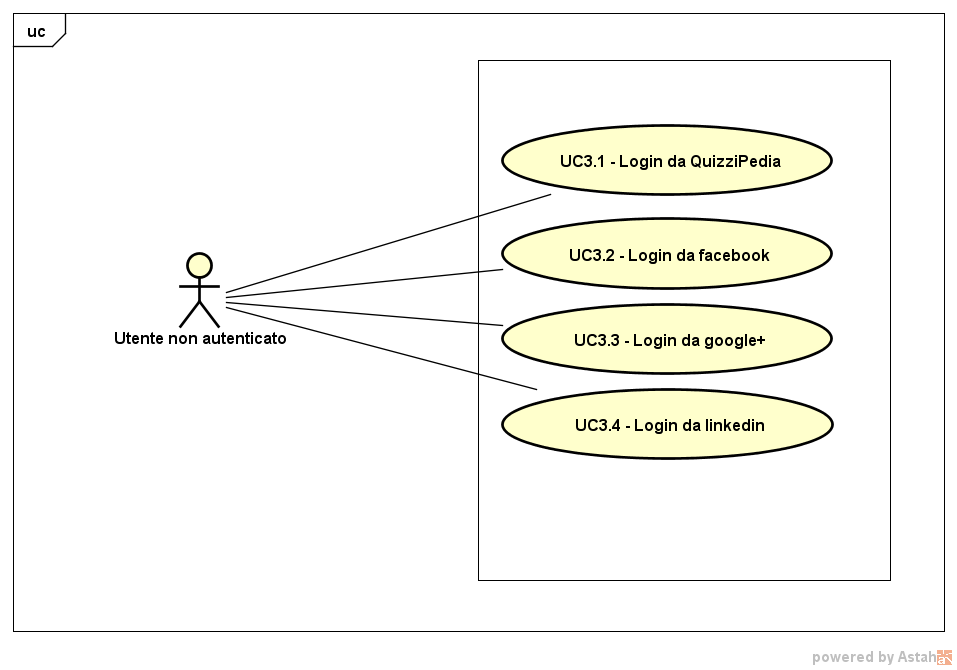
\includegraphics[scale=0.5]{UML/UC3.png}
	\end{center}
	\begin{itemize}
		\item
			\textbf{Attori}: Utente autenticato;
		\item		
			\textbf{Scopo e descrizione}: L'utente autenticato termina la sua sessione, uscendo dalla sua area riservata;
		\item
			\textbf{Pre-condizione}: L'utente è autenticato presso il sistema. 
		\item
			\textbf{Flusso principale degli eventi}:
	       		\begin{enumerate}
					\item 	
					L'Utente seleziona l'opzione logout per scollegarsi dal sistema [UC3.1];
					\item
					L'Utente riceve la conferma della disconnessione [UC3.2].
	 			\end{enumerate}
		\item
			\textbf{	Post-condizione}: L'utente non è autenticato presso il sistema.
	\end{itemize}

\subsubsection{Caso d'uso UC4.1: Selezione opzione logout}
	\begin{itemize}
		\item		
			\textbf{Attori}: Utente Autenticato;
		\item
  			\textbf{Scopo e descrizione}: L'utente seleziona l'opzione logout per poter uscire dalla sua area riservata;
		\item
			\textbf{Pre-condizione}: L'utente è autenticato presso il sistema. 
		\item
			\textbf{Post-condizione}: L'utente non è autenticato presso il sistema.
	\end{itemize}
\subsubsection{Caso d'uso UC4.2: Conferma disconnessione}
	\begin{itemize}
		\item
			\textbf{Attori}: Utente Autenticato;
		\item
			\textbf{Scopo e descrizione}: L'utente una volta selezionato l'opzione logout, attende la conferma della disconnessione da parte del sistema;
 		\item
			\textbf{Pre-condizione}: L'utente autenticato ha selezionato l'opzione logout;
		\item
			\textbf{Post-condizione}: Il sistema conferma all'utente l'uscita dalla sua area riservata.
	\end{itemize}		
	